\chapter{System Implementation}

This chapter details the system implementation for the project.
Section~\ref{sec:im:arch} covers the implemented system architecture, while
Section~\ref{sec:im:code} details the implemented code base for the integrated
system. Finally, Section~\ref{sec:im:summ} summarises the contributions
made by the author in implementing the project.

The implementation shall satisfy all the requirements laid out in
Section~\ref{sec:in:obj}.

The source code for the system has been uploaded to GitHub~\cite{gh-magor};
GitHub also serves as the version control and issue management
system for the project~\cite{gh-magor-is}.

\section{System Architecture}\label{sec:im:arch}

This section describes the system architecture to realise the processing
pipelines. However before that, let us define some terminology specific
to our processing framework:

\begin{itemize}
    \item A \textit{module} is a self-contained piece of software to realise
    one component of a processing pipeline. Different modules are specified
    by unique \texttt{module\_id}'s.
    \item A \textit{procedure} is a collection of modules to realise a
    processing pipeline; it is defined by the modules and the order in which
    they are run. Different procedures are specified by unique
    \texttt{procedure\_id}'s; they might have overlapping modules depending
    on procedure design.
    \item A \textit{process} is a specific configuration of procedures; in
    different processes the specific procedure's modules could have different
    versions. The processes provide the basic version mechanism to satisfy
    the requirements in Section~\ref{sec:in:obj}; different processes are
    specified by unique \texttt{process\_id}'s.
\end{itemize}

With that, we define our system architecture of the following four components:

\begin{itemize}
    \item \textit{Data} --- the source and generated files from the various
    processing pipelines
    \item \textit{Modules} --- the core processing functionalities
    \item \textit{Manifests} --- the specific system configurations
    \item \textit{System Executable} --- the executable linking data and
    modules; runs according to the manifests and generating module calls on
    data
\end{itemize}

Figure~\ref{top-arch} describes the high-level description of the interaction
between these four components, and figure~\ref{top-lvl} provides the top-level
folder structure of the system.

\begin{figure}[ht]
\begin{center}
    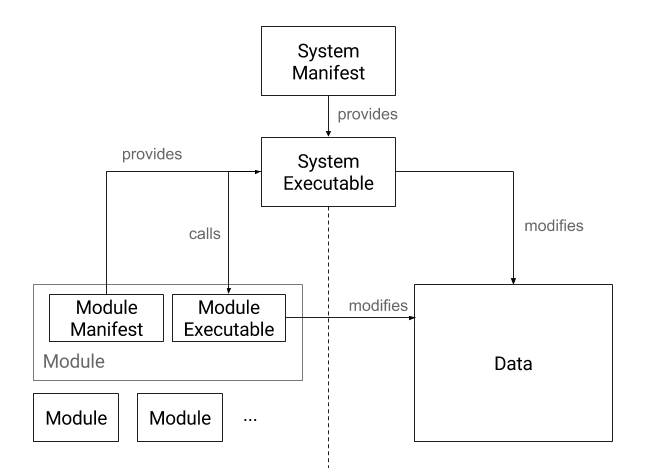
\includegraphics[width=0.9\textwidth]{system}
    \caption{High-level system architecture}\label{top-arch}
\end{center}
\end{figure}

\begin{figure}[ht]
\begin{lstlisting}
    crawl/
        --raw files--
    data/
        --data files--
    modules/
        --module files--
    system.py               # system executable
    manifest.json           # system manifest
\end{lstlisting}
\caption{Top-level folder structure}\label{top-lvl}
\end{figure}

The whole system would be implemented in Python, using JSON as the manifest
format owing to its inclusion in the Python standard library. The four
components would be described in detail in the following subsections.

\subsection{Data}\label{sec:im:arch:data}

The data used in the system are of two types. The first type is raw data, 
which are unprocessed audio or video files; these files are stored under
\texttt{crawl/}. The second type is processed data, which are stored under
\texttt{data/} in a specialised folder structure specified in Figure~\ref{data}:

\begin{figure}[ht]
\begin{lstlisting}
    data/
        process_id/
            file_id/
                raw/
                    --the raw file--
                module_1/
                    --output for module 1--
                module_2/
                    --output for module 2--
                ...
                module_n/
                    --output for module n--
                temp/
                    module_1/
                        --temporary files for module 1--
                    ...
\end{lstlisting}   
\caption{Data folder structure}\label{data} 
\end{figure}

Under this folder structure, the data is defined at the process and file level;
for each operation, the working folder (\texttt{working\_dir}) is set at
\texttt{data/process\_id/file\_id}, where \texttt{file\_id} denotes a unique
file identifier. This working folder would store all files associated with all
the modules in the respective process' procedures.

The data cycle could be seen as follows:

\begin{itemize}
    \item At system startup the system executable imports the raw file from
    \texttt{crawl/} into the \texttt{working\_dir/raw/} subfolder
    \item As a procedure is being executed, individual module's output files
    would be stored in the respective subfolder under \texttt{working\_dir},
    \item while the module's temporary files would be stored under
    \texttt{working\_dir/temp}
\end{itemize}

This structure allows the system to be fully modular; any module would only need
to know its own folder to dump íts output, and practically any operation could
be traced to the module level. Individual modules would be responsible in
implementing this structure.

\subsection{Modules}

All modules in the system are placed under the subfolder \texttt{modules/}
according to the folder structure described in Figure.
Each module has its own folder; the folder name is a module identifier in
the form of \texttt{module\_name-version}. This allows multiple versions of
a module to co-exist in the system. In each module folder there are three
compulsory components --- a \texttt{setup} script to setup the module and all
its dependencies, a Python executable \texttt{module.py} to call the module,
and a manifest file\footnote{The structure of this file would be detailed later
in the section on Manifests.} in JSON format to specify the module details.
The module setup script and executable could be run independently of the system
for development and testing purposes; this also ensures self-containment of the
module.

\begin{figure}[ht]
\begin{lstlisting}
    modules/
        module_id_1/
            setup           # module setup script
            module.py       # module executable
            manifest.json   # module manifest
            --optional module data and executables--
        module_id_2/
            ...
        ...            
\end{lstlisting}
\caption{Module folder structure}\label{module}
\end{figure}

\subsection{Manifests}

There are two types of manifest in the implemented system --- modular manifest
and system manifest. Both types provide configuration options that are not
hard-coded into the system, allowing easy maintenance and upgrade.

\subsubsection{Modular manifests}

Each module has its own manifest, at the path \texttt{module\_id/manifest.json}
as specified in Figure~\ref{module}. The manifest file must conform to the
JSON structure specified in Figure~\ref{manifest-md}.

\begin{figure}[ht]
\begin{lstlisting}
    {
        "name": "module_name",
        "version": "module_version",
        "requires": [],
        "inputs": [],
        "outputs": []
    }
\end{lstlisting}
\caption{Modular manifest structure}\label{manifest-md}
\end{figure}

\texttt{requires}, \texttt{inputs} and \texttt{outputs} are all JSON lists.
\texttt{requires} is a list of (optional) data files and executables required
for the module's functionality; these files should be in place after running
the \texttt{setup} script. \texttt{inputs} and \texttt{outputs} are lists of
subfolders under \texttt{working\_dir}\footnote{See Section~\ref{sec:im:arch:data}
on Data.} where the module would pull its input files and push its output
files, respectively.

In this way, the manifest file serves as a blueprint of the module to the
system; this blueprint would be realised by the module executable.

\subsubsection{System manifest}

The system manifest specifies system-level properties; specifically the
processes, procedures and the file formats accepted by the system. It follows
the structure described in Figure~\ref{manifest-sys}; the fields' properties
are described in Table~\ref{table:manifest-sys}.

\begin{figure}[ht]
\begin{lstlisting}
    {
        "processes": {
            "process_id_1":{
                "module_id_1": "version",
                "module_id_2": "version",
                ...
            },
            ...
        }
        "default_process": "process_id",
        "procedures": {
            "procedure_id_1": [
                "module_name_1",
                "module_name_2",
                ...
            ],
            ...
        },
        "default_procedures": [],
        "file_types": {
            "audio": [],
            "video": []
        }
    }
\end{lstlisting}
\caption{System manifest structure}\label{manifest-sys}
\end{figure}

\begin{longtabu}{X[1.5,l]X[3.5,l]X[1,l]}
    \textbf{Field} & \textbf{Description} & \textbf{Type} \\
    \midrule
    \endhead{}
    \texttt{processes} &
    The processes in the system, specified by the module versions &
    \texttt{dict} \\
    \texttt{default\_process} &
    The default \texttt{process\_id} (if no process is specified to run,
    this process would be executed) &
    \texttt{str} \\
    \texttt{procedures} &
    The procedures in the system, specified by a list of module names &
    \texttt{dict} \\
    \texttt{default\_procedures} &
    The default \texttt{procedure\_id}'s (if no procedure is specified to
    run, these procedures would be executed) &
    \texttt{list\,(str)} \\
    \texttt{file\_types} &
    The file extensions accepted by the system &
    \texttt{dict} \\
    \caption{System manifest fields}\label{table:manifest-sys}
\end{longtabu}

In this way, the system manifest provides a blueprint of the whole system
to the system executable.

\subsection{System executable}

The system executable links the modules and data together by issuing module
calls on the data, given the manifest. A system run would proceed as follows:

\begin{itemize}
    \item Startup manifest checks --- load all manifests, perform error
    checks and eliminate invalid manifest items
    \item File import --- import the correct files from \texttt{crawl/}
    into the data structure in
    \texttt{data/}\footnote{See Section~\ref{sec:im:arch:data} on Data.}
    \item Pipeline --- call the modules in the procedure one-by-one in
    the order specified by the system manifest
\end{itemize}

\subsection{Evaluation of System Architecture}

The current system architecture described is able to satisfy three out of
five qualitative requirements outlined in Section~\ref{sec:in:obj}:

\begin{itemize}
    \item Modularity --- the well-defined components are independent and
    exhibits low coupling
    \item Extensibility --- the use of manifests allows for easy extension
    of system; components could be added independently of existing
    components and the system executable
    \item Versioning --- explicit versioning through the use of processes
    and different working folders per process
\end{itemize}

The next section would detail the code base implemented for the project,
which would address the primary objectives and the remaining qualitative
requirements.

\section{Implemented Code Base}\label{sec:im:code}

\section{Summary}\label{sec:im:summ}